\clearpage
\subsection{Countdown Test Runs} % (fold)
\label{sub:countdown_test_runs}
This section displays the test runs for the countdown screen.

\subsubsection{Displays Remaining Time} % (fold)
\label{ssub:displays_remaining_time}
\begin{figure}[!htbp]
\centering
\begin{subfigure}{0.5\textwidth}
  \centering
  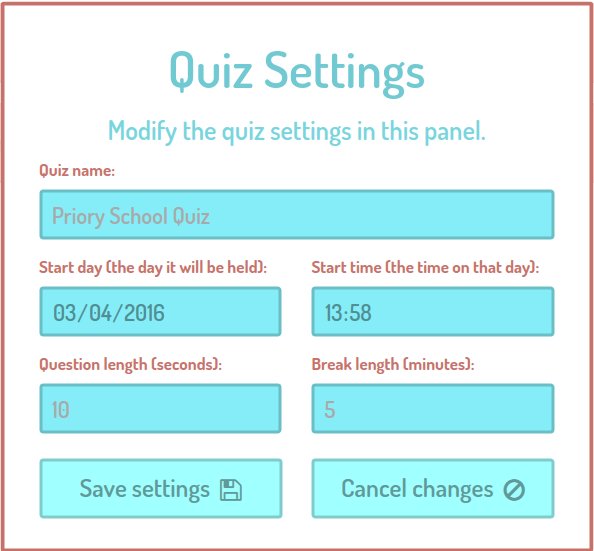
\includegraphics[width=0.95\linewidth]{testing/countdown/schedule}
  \caption{Scheduling the quiz for 10 minutes}
  \label{fig:sub1}
\end{subfigure}%
\begin{subfigure}{0.5\textwidth}
  \centering
  
\includegraphics[width=0.95\linewidth]{testing/countdown/10}
  \caption{The countdown immediately afterwards.}
  \label{fig:sub2}
\end{subfigure}
\begin{subfigure}{0.5\textwidth}
  \centering
  
\includegraphics[width=0.95\linewidth]{testing/countdown/3}
  \caption{The countdown seven minutes later.}
  \label{fig:sub3}
\end{subfigure}
\caption{Countdown showing the correct time.}
\label{fig:test}
\end{figure}
As the figures show, the countdown screen successfully displays the correct time remaining until the quiz begins. \textit{Success.}
% subsubsection displays_remaining_time (end)

\subsubsection{Begins Quiz at Correct Time} % (fold)
\label{ssub:begins_quiz_at_correct_time}
This test is covered under the navigation section owing to its difficulty to prove using screenshots.
% subsubsection begins_quiz_at_correct_time (end)
% subsection countdown_test_runs (end)
